\chapter{Experimentación}\label{chap:experiments}
Los experimentos realizados sobre las implementaciones mencionadas en el capítulo anterior tienen como objetivo comparar el tiempo de ejecución de los algoritmos en sus distintas variantes de implementación.
Se realizaron varios experimentos preliminares para analizar cómo los parámetros de cada estructura utilizada puede alterar el tiempo de ejecución.
Por ejemplo, realizamos un análisis del rendimiento de un \mintinline{haskell}{LockFreeStack} según sus distintos parámetros (tiempos límites mínimos y máximos de backoff) para luego usar la configuración óptima al momento de comparar el rendimiento de la estructura con las demás.
Luego, se realizaron los tres experimentos comparando las estructuras, alterando las variables de control para obtener resultados en los cuales se pudieron apreciar tendencias significativas y así realizar un análisis comprensivo.

\section{Detalle de los experimentos}\label{sec:experiment-details}

La experimentación consiste en comparar los tiempos de ejecución de un programa Haskell para determinar cuales implementaciones obtienen un mejor rendimiento en tiempo de ejecución respecto de las demás.
Cada programa será ejecutado varias veces para luego realizar un promedio y poder obtener una apreciación de la consistencia de los resultados con diagramas \emph{boxplot}.
Los experimentos realizados fueron tres.
Uno estudia cómo varía el tiempo de ejecución respecto de la variación de la proporción de hilos escritores representado en el valor de la variable \mintinline{haskell}{pushPercentages}.
Los otros dos estudian cómo la variación de la cantidad de hilos totales afecta el tiempo de ejecución pero con una distinción, en un experimento la cantidad de operaciones, representada por la variable \mintinline{haskell}{operationCount}, es distribuída entre los hilos mientras que en el otro es la cantidad de operaciones que cada hilo debe realizar.
A continuación se listan los nombres utilizados para identificar a los experimentos:

\begin{itemize}
    \item \mintinline{haskell}{pushPercentages}: proporción de hilos escritores vs. tiempo de ejecución.
    \item \mintinline{haskell}{numberOfThreads}: cantidad de hilos vs. tiempo de ejecución. En este caso la cantidad de operaciones totales aumenta ya que cada hilo debe realizar una cantidad de operaciones igual al parámetro \mintinline{haskell}{operationCount}
    \item \mintinline{haskell}{numberOfThreadsDist}: mismo análisis que \mintinline{haskell}{numberOfThreads} con la distinción que la cantidad de total de operaciones realizada se mantiene constante para cada cantidad de hilos. Es decir, el parámetro \mintinline{haskell}{operationCount} establece el número de operaciones totales y estas son distribuídas equitativamente según la cantidad de hilos que haya.
\end{itemize}

\subsection{Hipótesis}\label{subsec:hypothesis}
La hipótesis manejada fue que la implementación STM \mintinline{haskell}{StackSTM} superaría a varias, si no todas, de las demás implementaciones ya que ha habido mucho trabajo sobre el compilador GHC para poder mejorar la performance de STM.
Unos resultados parecidos se encuentran en \hl{ref a paper-abq} dónde se comparan dos implementaciones de una misma estructura, una utilizando STM y la otra utilizando algoritmos que utilizan locks sobre la estructura de datos.
En este trabajo, los resultados muestran que la implementación STM supera a la otra a medida que aumenta la cantidad de núcleos a utilizar por el procesador entre cada corrida.

También estuvieron en consideración los resultados de \hl{ref a paper-linked-list} donde se comparan implementaciones similares de una lista simplemente encadenada.
En estos resultados, la implementación sobre STM no obtiene buenos tiempos de ejecución comparado al resto.
Sin embargo, esto se debe a que en una lista encadenada, uno la debe recorrer y esto resulta en muchas llamadas a la función \mintinline{haskell}{atomically} para recorrer la lista.
En el caso de la implementación de \mintinline{haskell}{StackSTM}, cada operación realiza una sola llamada a \mintinline{haskell}{atomically}, ya que las operaciones trabajan sólamente con el tope de la pila, y es por eso que no esperamos resultados similares a \hl{ref a linked list}.

\subsection{Instrumentación para realizar los experimentos}\label{subsec:experiment-harness}
Las implementaciones comparadas en los experimentos son \mintinline{haskell}{LockFreeStackIO}, \mintinline{haskell}{LockFreeStackSTM}, \mintinline{haskell}{EliminationBackoffStackIO}, \mintinline{haskell}{EliminationBackoffStackSTM}, y \mintinline{haskell}{StackSTM}. Para cada una de ellas, tendremos un programa Haskell tomará los siguientes parámetros por línea de comando:

\begin{itemize}
    \item \mintinline{haskell}{min} y \mintinline{haskell}{max}: Los parámetros para la estructura \mintinline{haskell}{LockFreeStack}. Estos consisten de los límites mínimos y máximos de la estructura de backoff que se encuentra detallada en la subsección \ref{sub:backoff}.
    \item \mintinline{haskell}{count} y \mintinline{haskell}{duration}: Los parámetros para la estructura \mintinline{haskell}{EliminationBackoffStack}. Estos son la capacidad del \mintinline{haskell}{EliminationArray} y la duración del timeout a pasar por parámetro en las llamdas a la función \mintinline{haskell}{exchange} de cada \mintinline{haskell}{LockFreeExchanger}.
    \item \mintinline{haskell}{threadCount}: Cantidad de hilos de ejecución que serán creados para operar sobre una pila.
    \item \mintinline{haskell}{distributeOperations}: un valor booleano que determina si el parámetro \mintinline{haskell}{operationCount} se interpreta como la cantidad total de operaciones a ser distribuida entre los hilos o la cantidad que cada hilo debe realizar por separado.
    \item \mintinline{haskell}{operationCount}: Cantidad de operaciones a realizar en el experimento. Estas pueden ser cantidad de operaciones por hilo, o cantidad de operaciones totales que luego serán distribuidas entre la cantidad de hilos según el experimento.
    \item \mintinline{haskell}{pushPercentage}: La proporción de hilos que realizarán operaciones de escritura (\mintinline{haskell}{push}). Se tomará la cantidad de hilos de ejecución y se calculará la cantidad de hilos que realizarán operaciones de escritura sobre la pila según la proporción, el resto realizará operaciones de lectura (\mintinline{haskell}{pop}).
\end{itemize}

El programa se encarga de crear una instancia de pila según la implementación y sus parámetros, luego inserta 100000 elementos para evitar que ocurran excepciones por pila vacía durante la ejecución.
Una vez instanciada la pila, se calcula la cantidad de threads escritores que se deben crear según la proporción dada por \mintinline{haskell}{pushPercentage} sobre \mintinline{haskell}{threadCount} y la cantidad de operaciones que debe realizar cada hilo tomando en cuenta los parámetros \mintinline{haskell}{operationCount} y \mintinline{haskell}{distributeOperations}.
Finalmente se inicia un reloj al crear los hilos escritores y lectores para que realicen sus operaciones y al finalizar todos los hilos se imprime por pantalla la cantidad de tiempo en segundos transcurrido.
A continuación se presenta el código Haskell del programa para la implementación \mintinline{haskell}{EliminationBackoffStackIO} en la Fig. \ref{fig:expEBSIO}.

\begin{figure}[H]
    \centering
    \begin{minted}[linenos,breaklines,fontsize=\footnotesize]{haskell}
callPushes stack operationCount = do
    if operationCount > 0
        then do
            (randomIO :: IO Int) >>= pushEBSIO stack
            callPushes stack (operationCount - 1)
        else do
            return ()

callPops stack operationCount = do
    if operationCount > 0
        then do
            _ <- catch (popEBSIO stack) (\(e :: EmptyException) -> return 1)
            callPops stack (operationCount - 1)
        else do
            return ()

threadAction isPushThread = if isPushThread then callPushes else callPops

createThreads stack threadCount pushThreadCount operationCount tids = do
    let isPushThread = if pushThreadCount > 0 then True else False
    if threadCount > 0
        then do
            tid <- async (threadAction isPushThread stack operationCount)
            createThreads stack (threadCount - 1) (pushThreadCount - 1) operationCount (tid : tids)
        else
            mapM_ wait tids

parseCommandLineArguments args = do
    -- Get arguments from command line
    capacity <- readIO (args !! 0) :: IO Int
    duration <- readIO (args !! 1) :: IO Integer
    operationCount <- readIO (args !! 2) :: IO Int
    pushPercentage <- readIO (args !! 3) :: IO Float
    threadCount <- readIO (args !! 4) :: IO Int
    distributeOperations <- readIO (args !! 5) :: IO Bool
    -- Distribute operationCount
    operationCount <- return $ if distributeOperations then quot operationCount threadCount else operationCount
    -- Create stack and calculate amount of writer/push threads
    stack <- newEBSIO capacity duration
    let pushThreadCount = floor $ (fromIntegral threadCount :: Float) * pushPercentage
    return (stack, threadCount, operationCount, pushThreadCount)

main = do
    args <- getArgs
    (stack, threadCount, operationCount, pushThreadCount) <- parseCommandLineArguments args
    callPushes stack 1000000
    timeIt "" $ createThreads stack threadCount pushThreadCount operationCount []
    return ()
    \end{minted}
    \caption{Código Haskell para la experimentación sobre la implementación \mintinline{haskell}{EliminationBackoffStackIO}}
    \label{fig:expEBSIO}
\end{figure}

% Fijarse los números de líneas para dejar en claro en qué líneas hay renombre por funciones de otras implementaciónes

Cada uno de los tres experimentos tienen un script bash para ejecutar los programas Haskell variando los parámetros de acorde al experimento, la implementación de pila deseada, y también la cantidad de núcleos del procesador.
Una vez determinada la combinación implementación-cantidad de núcleos, se ejecuta el programa Haskell de manera que la variación de parámetros coincida con lo que se quiere observar del experimento.
Es decir, si el experimento en cuestión busca estudiar cómo la proporción de hilos escritores varía el tiempo de ejecución, el script bash se encargará de ejecutar, para cada combinación de implementación-cantidad de núcleos, el programa Haskell de esa implementación variando el valor del parámetro \mintinline{haskell}{pushPercentages} y manteniendo el resto constantes.
Para cada valor que puede tomar la variable \mintinline{haskell}{pushPercentages} en este ejemplo, se realizarán varias corridas del mismo programa Haskell y se escribirán los resultados en un archivo CSV para cada combinación implementación-cantidad de núcleos.
Luego los scripts llaman a un programa Python que creará los gráficos partiendo de los archivos CSV escritos anteriormente.

\section{Resultados}\label{sec:results}

% Agregar una referencia a la página de Apple con las especificaciones
Los experimentos fueron realizados utilizando una laptop MacBook Pro del año 2016 con las siguientes especificaciones:

\begin{itemize}
    \item \textbf{Procesador}: 2.0GHz dual-core Intel Core i5, Turbo Boost up to 3.1GHz, with 4MB shared L3 cache
    \item \textbf{Memoria}: 16 GB 1867 MHz LPDDR3
    \item \textbf{Sistema operativo}: macOS Mojave, versión 10.14
\end{itemize}

Dado que el equipo en cuestión tiene un procesador con cuatro núcleos, nuestros experimentos fueron limitados a ser realizados utilizando uno, dos, y cuatro núcleos.

\subsection{Primer experimento: \mintinline{haskell}{pushPercentages}}\label{subsec:pushPercentages}

\clearpage
\subsection{Segundo experimento: \mintinline{haskell}{numberOfThreads}}\label{subsec:numberOfThreads}
Para este experimento se analizó el comportamiento del tiempo de ejecución a medida que se aumentaron la cantidad de hilos de ejecución y la cantidad de operaciones totales.
Las variables constantes tomaron los siguientes valores:

\begin{itemize}
    \item Proporción de hilos escritores: 0.75
    \item Cantidad de operaciones realizadas por hilo de ejecución: 10000
    \item Límite mínimo de backoff para las implementaciones de LFS: 100
    \item Límite máximo de backoff para las implementaciones de LFS: 1000
    \item Capacidad del \mintinline{haskell}{EliminationArray} para las implementaciones de EBS: 1
    \item Duración del timeout para las implementaciones de EBS: 100
    \item Cantidad de repeticiones de cada corrida: 10
\end{itemize}

En este experimento, a medida que incrementa la cantidad de hilos, la cantidad de operaciones totales realizadas sobre la pila incrementa ya que cada hilo nuevo realiza unas 10000 operaciones adicionales sobre la pila.

\begin{figure}[H]
    \centering
    \begin{subfigure}[b]{0.49\textwidth}
        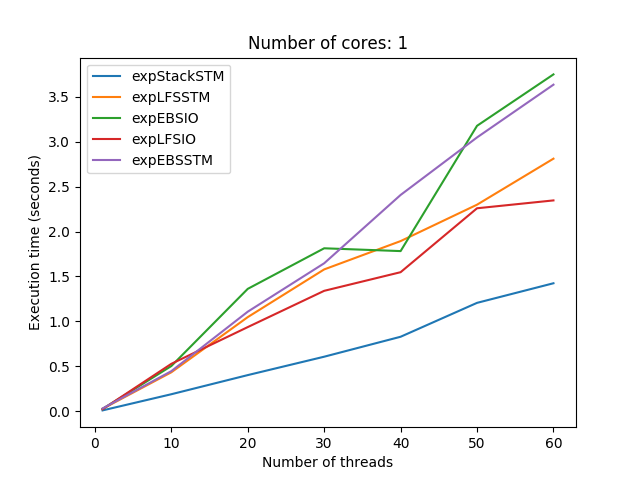
\includegraphics[width=\textwidth]{images/numberOfThreads/plots/1.png}
        \caption{1 núcleo}
        \label{subfig:numberOfThreads-1core}
    \end{subfigure}
    ~
    \begin{subfigure}[b]{0.49\textwidth}
        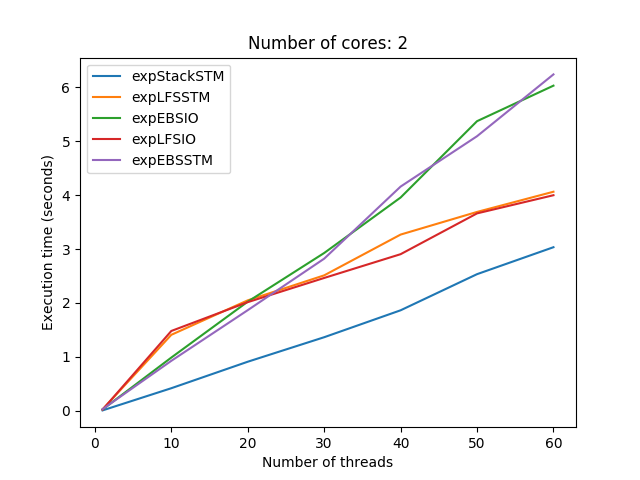
\includegraphics[width=\textwidth]{images/numberOfThreads/plots/2.png}
        \caption{2 núcleos}
        \label{subfig:numberOfThreads-2core}
    \end{subfigure}
    ~
    \begin{subfigure}[b]{0.5\textwidth}
        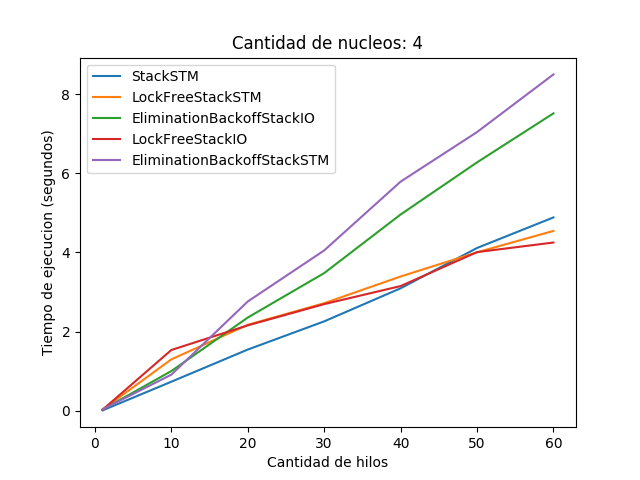
\includegraphics[width=\textwidth]{images/numberOfThreads/plots/4.png}
        \caption{4 núcleos}
        \label{subfig:numberOfThreads-4core}
    \end{subfigure}
    \caption{Resultados para el experimento \mintinline{haskell}{numberOfThreads}}
    \label{fig:numberOfThreads-all}
\end{figure}

Se pueden observar resultados similares en los tres gráficos. Una diferencia es que cuando los experimentos son ejecutados utilizando cuatro núcleos del procesador, la implementación \mintinline{haskell}{StackSTM} no resulta ser la óptima y al aumentar la cantidad de hilos de ejecución resulta tardar más que las implementaciones de LFS como muestra la subfigura \ref{subfig:numberOfThreads-4core}.
En la misma subfigura, vemos que la implementación de EBS sobre IO supera a la implementación sobre STM mientras que en el caso de 1 y 2 núcleos, ambas implementaciones no presentan diferencias considerables en tiempo de ejecución.

Para realizar un análisis más profundo de los experimentos, se analizaron los resultados de las corridas y se generaron gráficos con diagramas \emph{boxplot} para apreciar la consistencia de cada implementación en cuanto a los tiempos de ejecución que logra a través de las corridas repetidas. Estos gráficos se encuentran en la Fig. \ref{fig:numberOfThreads-boxplots}.

En la figura \ref{fig:numberOfThreads-boxplots} se muestran los resultados para cada implementación utilizando dos núcleos del procesador.
En las subfiguras se presentan diagramas \emph{boxplot} que representan el rango de valores que resultaron de correr el programa Haskell en múltiples iteraciones.
La cantidad de veces que la corrida fue repetida está determinada por el parámetro \mintinline{haskell}{iterations}. Observando los gráficos, se puede ver que los resultados para la implementación \mintinline{haskell}{StackSTM} tienen diagramas \emph{boxplot} de menor rango, lo cual infiere una mayor consistencia para producir los mismos resultados al repetir el experimento.
La implementación que parece ser la menos consistente son las implementaciones de LFS, tanto IO como STM, donde se ven boxplots de mayor rango.
En el caso de las implementaciones de EBS, observamos también diagramas \emph{boxplot} consistentes, aunque se pueden distinguir anomalías en los resultados, como por ejemplo, en la Subfig. \ref{subfig:numberOfThreads-ebsio-2} dónde se encuentra un resultado por encima de los 8 segundos.

\clearpage
\begin{figure}[H]
    \centering
    \begin{subfigure}[b]{0.49\textwidth}
        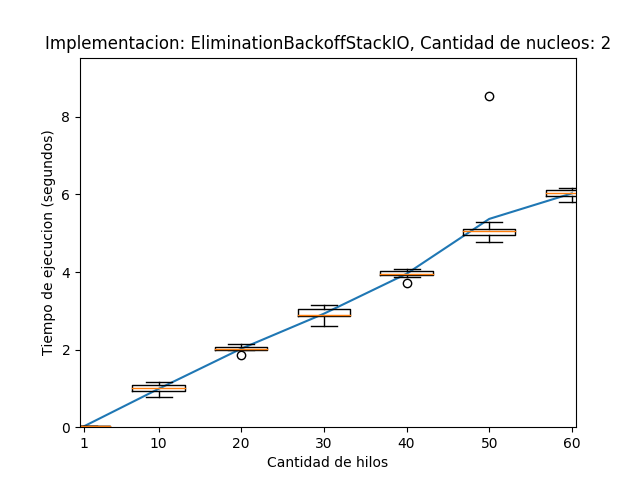
\includegraphics[width=\textwidth]{images/numberOfThreads/plots/expEBSIO-2}
        \caption{Resultados para EBS sobre IO}
        \label{subfig:numberOfThreads-ebsio-2}
    \end{subfigure}
    ~
    \begin{subfigure}[b]{0.49\textwidth}
        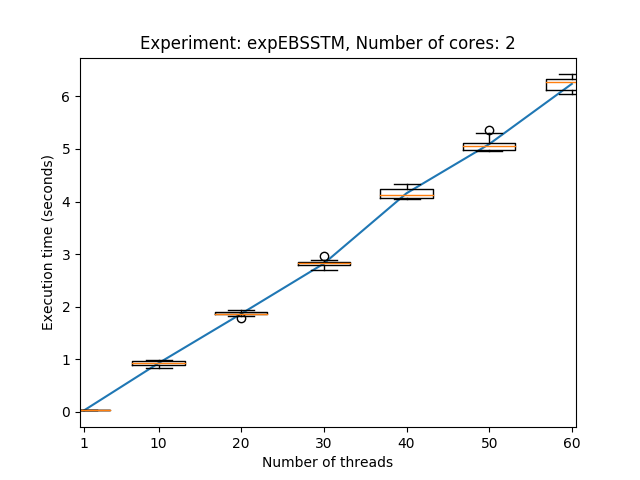
\includegraphics[width=\textwidth]{images/numberOfThreads/plots/expEBSSTM-2}
        \caption{Resultados para EBS sobre STM}
        \label{subfig:numberOfThreads-ebsstm-2}
    \end{subfigure}
    \begin{subfigure}[b]{0.49\textwidth}
        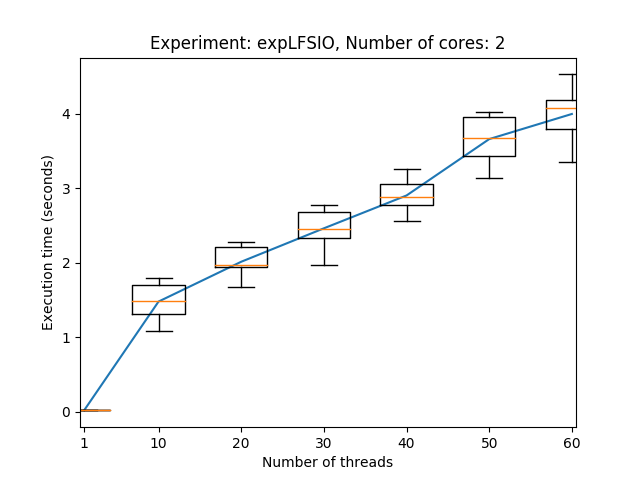
\includegraphics[width=\textwidth]{images/numberOfThreads/plots/expLFSIO-2}
        \caption{Resultados para LFS sobre IO}
        \label{subfig:numberOfThreads-lfsio-2}
    \end{subfigure}
    ~
    \begin{subfigure}[b]{0.49\textwidth}
        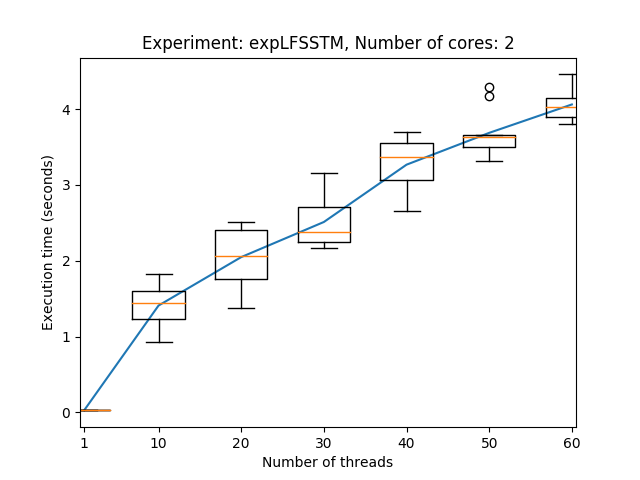
\includegraphics[width=\textwidth]{images/numberOfThreads/plots/expLFSSTM-2}
        \caption{Resultados para LFS sobre STM}
        \label{subfig:numberOfThreads-lfsstm-2}
    \end{subfigure}
    \begin{subfigure}[b]{0.49\textwidth}
        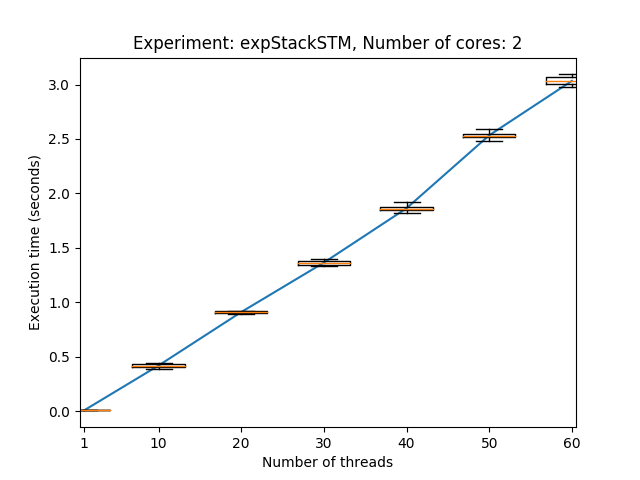
\includegraphics[width=\textwidth]{images/numberOfThreads/plots/expStackSTM-2}
        \caption{Resultados para LFS sobre STM}
        \label{subfig:numberOfThreads-stackstm-2}
    \end{subfigure}
    \caption{Comparación de implementaciones IO vs STM del experimento \mintinline{haskell}{numberOfThreads}}
    \label{fig:numberOfThreads-boxplots}
\end{figure}



% TODO: Agregar comentario sobre que más resultados como estos se pueden encontrar en un apéndice

\clearpage
\subsection{Tercer experimento: \mintinline{haskell}{numberOfThreadsDist}}
Para este experimento se analizó el comportamiento del tiempo de ejecución a medida que se aumentaron la cantidad de hilos de ejecución mantienendo constante la cantidad total de operaciones realizadas sobre la pila.
Las variables constantes tomaron los siguientes valores:

\begin{itemize}
    \item Proporción de hilos escritores: 0.75
    \item Cantidad de operaciones totales: 1000000
    \item Límite mínimo de backoff para las implementaciones de LFS: 100
    \item Límite máximo de backoff para las implementaciones de LFS: 1000
    \item Capacidad del \mintinline{haskell}{EliminationArray} para las implementaciones de EBS: 1
    \item Duración del timeout para las implementaciones de EBS: 100
    \item Cantidad de repeticiones de cada corrida: 10
\end{itemize}

A diferencia del experimento en la subsección \ref{subsec:numberOfThreads}, en este experimento se mantiene constante la cantidad de operaciones totales.
Es decir, a medida que incrementa la cantidad de hilos de ejecución, la cantidad de operaciones se distribuye equitativamente entre los distintos hilos.

Los resultados presentes en la Fig. \ref{fig:numberOfThreadsDist-all} muestran tendencias similares a los experimentos anteriores.
Se mantiene que la implementación con mejores tiempos de ejecución es la de \mintinline{haskell}{StackSTM} para uno y dos núcleos, mientras que en el caso de cuatro núcleos es superada por las implementaciones de LFS.
En este último caso, la diferencia de tiempos entre las implementaciones LFS y la de \mintinline{haskell}{StackSTM} es más notoria que en los experimentos anteriores.



\clearpage
\begin{figure}[H]
    \centering
    \begin{subfigure}[b]{0.49\textwidth}
        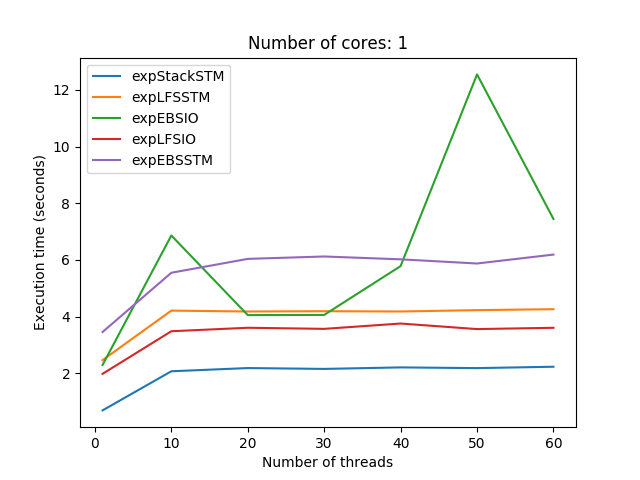
\includegraphics[width=\textwidth]{images/numberOfThreadsDist/plots/1.png}
        \caption{1 núcleo}
        \label{subfig:numberOfThreadsDist-1core}
    \end{subfigure}
    ~
    \begin{subfigure}[b]{0.49\textwidth}
        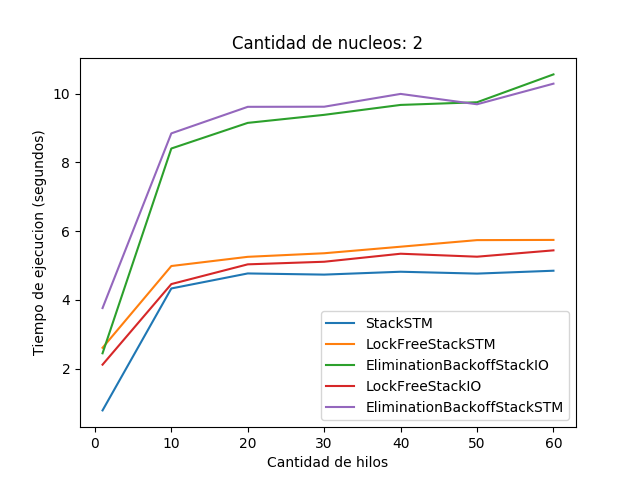
\includegraphics[width=\textwidth]{images/numberOfThreadsDist/plots/2.png}
        \caption{2 núcleos}
        \label{subfig:numberOfThreadsDist-2core}
    \end{subfigure}
    ~
    \begin{subfigure}[b]{0.5\textwidth}
        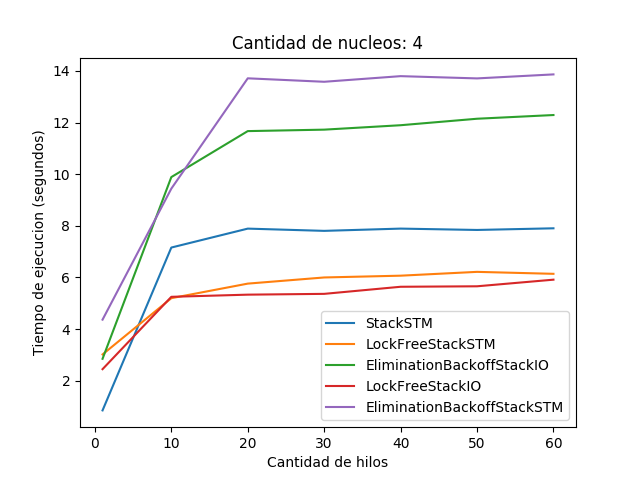
\includegraphics[width=\textwidth]{images/numberOfThreadsDist/plots/4.png}
        \caption{4 núcleos}
        \label{subfig:numberOfThreadsDist-4core}
    \end{subfigure}
    \caption{Resultados para el experimento \mintinline{haskell}{numberOfThreadsDist}}
    \label{fig:numberOfThreadsDist-all}
\end{figure}

Las tendencias parecen indicar que a medida que aumenta la cantidad de hilos el tiempo de ejecución se mantiene dentro de un mismo rango de valores a partir de los 10 hilos de ejecución. Esto se puede ver en las subfiguras de la Fig. \ref{fig:numberOfThreadsDist-all} dónde las líneas no tienen cambios considerables en la tendencia a partir de 10 hilos.
Sin embargo, se observa un comportamiento errático para los tiempos de ejecución de la implementación de EBS sobre IO cuando se corre el programa sobre un núcleo del procesador.
Para observar este caso en más detalle, se presenta la siguiente Fig. \ref{fig:numberOfThreadsDist-EBSIO} donde se muestra los diagramas \emph{boxplot} para los resultados de la implementación de EBS sobre IO con un núcleo del procesador.

\clearpage
\begin{figure}[H]
    \centering
    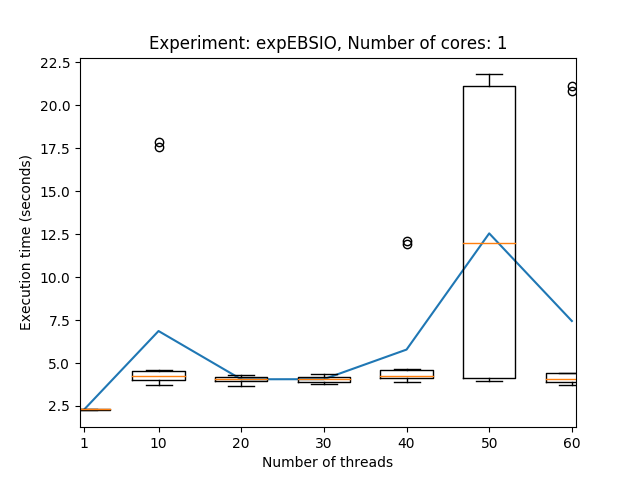
\includegraphics[width=0.5\textwidth]{images/numberOfThreadsDist/plots/expEBSIO-1.png}
    \caption{Resultados del experimento \mintinline{haskell}{numberOfThreadsDist} para EBS sobre IO}
    \label{fig:numberOfThreadsDist-EBSIO}
\end{figure}

Una vez más, se puede apreciar que la implementación sobre IO de EBS ha presentado irregularidades en sus resultados en la forma de \emph{outliers} o el rango del boxplot en los resultados con 50 hilos de ejecución.
Estas irregularidades son la causa de la tendencia presentada en la subfigura \ref{subfig:numberOfThreadsDist-1core}.
A continuación se presentan el resto de los gráficos individuales de cada implementación con los diagramas \emph{boxplot} para cada valor en la Fig. \ref{fig:numberOfThreadsDist-boxplots}.

\clearpage
\begin{figure}[H]
       \centering
    \begin{subfigure}[b]{0.49\textwidth}
        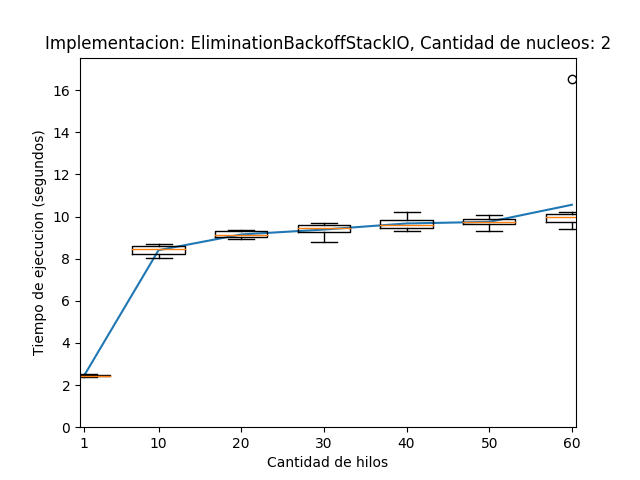
\includegraphics[width=\textwidth]{images/numberOfThreadsDist/plots/expEBSIO-2}
        \caption{Resultados para EBS sobre IO}
        \label{subfig:numberOfThreadsDist-ebsio-2}
    \end{subfigure}
    ~
    \begin{subfigure}[b]{0.49\textwidth}
        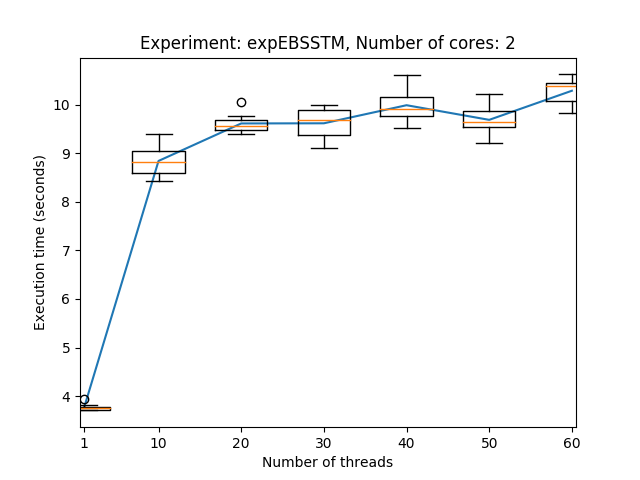
\includegraphics[width=\textwidth]{images/numberOfThreadsDist/plots/expEBSSTM-2}
        \caption{Resultados para EBS sobre STM}
        \label{subfig:numberOfThreadsDist-ebsstm-2}
    \end{subfigure}
    \begin{subfigure}[b]{0.49\textwidth}
        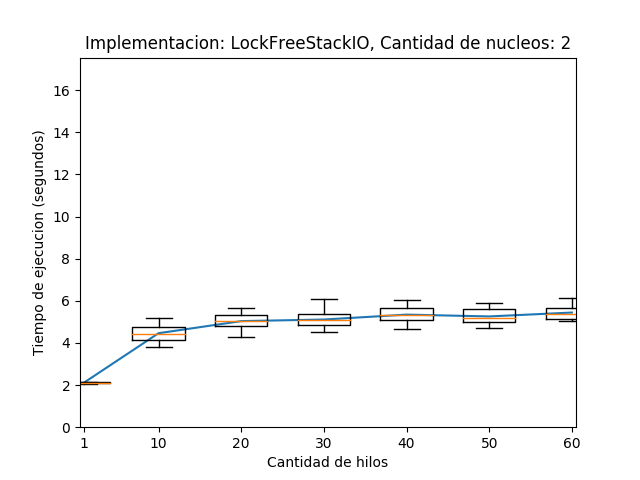
\includegraphics[width=\textwidth]{images/numberOfThreadsDist/plots/expLFSIO-2}
        \caption{Resultados para LFS sobre IO}
        \label{subfig:numberOfThreadsDist-lfsio-2}
    \end{subfigure}
    ~
    \begin{subfigure}[b]{0.49\textwidth}
        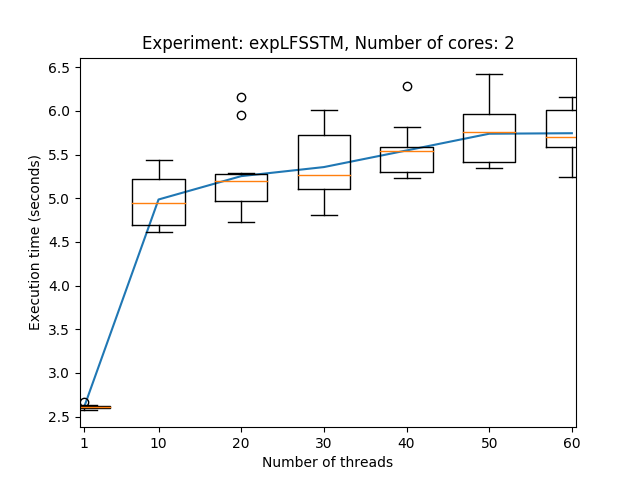
\includegraphics[width=\textwidth]{images/numberOfThreadsDist/plots/expLFSSTM-2}
        \caption{Resultados para LFS sobre STM}
        \label{subfig:numberOfThreadsDist-lfsstm-2}
    \end{subfigure}
    \begin{subfigure}[b]{0.49\textwidth}
        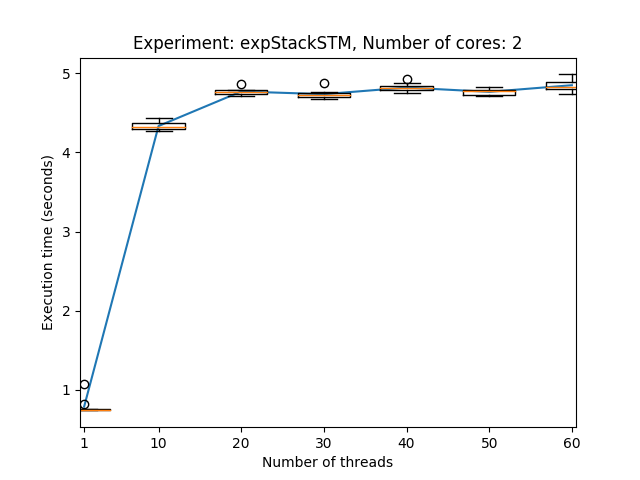
\includegraphics[width=\textwidth]{images/numberOfThreadsDist/plots/expStackSTM-2}
        \caption{Resultados para LFS sobre STM}
        \label{subfig:numberOfThreadsDist-stackstm-2}
    \end{subfigure}
    \caption{Comparación de implementaciones IO vs STM del experimento \mintinline{haskell}{numberOfThreadsDist}}
    \label{fig:numberOfThreadsDist-boxplots}
\end{figure}

En la Fig. \ref{fig:numberOfThreadsDist-boxplots} se puede apreciar cómo la implementación de \mintinline{haskell}{StackSTM} sigue siendo la que produce resultados más consistentes a medida que se repiten las corridas.
También se aprecia nuevamente la aparición de outliers en la implementación de EBS sobre IO, como por ejemplo el punto que se puede observar en la subfigura \ref{subfig:numberOfThreadsDist-ebsio-2} dónde una corrida con 60 hilos de ejecución tomó 16 segundos en completarse.
Se pueden observar outliers en otros gráficos como las subfiguras \ref{subfig:numberOfThreadsDist-lfsstm-2} y \ref{subfig:numberOfThreadsDist-ebsstm-2}, pero estos no se encuentran muy alejados del rango de su respectivo \emph{boxplot}.
